\chapter{Was ist ein DDoS-Angriff?}
\label{chap:kapitel1}
Die Grundlage für einen \ac{ddos}-Angriff ist ein \ac{dos}-Angriff. Ein \ac{dos}-Angriff (\acl{dos}-Angriff) hat das Ziel ein System nicht mehr verfügbar zu machen. Dazu kann entweder die begrenzte Bandbreite so ausgenutzt werden, dass die eigentlichen Nutzer des Systems dieses nicht mehr erreichen können. Eine andere Möglichkeit ist die Überlastung des Systems selbst (CPU, RAM, ...), damit dieses nicht mehr (zeitnah) antworten kann.

Solche Angriffe richten meist keinen permanenten Schaden an der IT-Infrastruktur direkt an. Ist der Angriff vorbei, so kann der Normalbetrieb in der Regel wieder aufgenommen werden. Dennoch können sie einen (erheblichen) finanziellen Schaden anrichten. Das gilt beispielsweise für Unternehmen, welche sehr stark auf den Verkauf ihrer Waren im Internet setzen. Eine Nichtverfügbarkeit würde hierbei enorme finanzielle Einbuße einbringen. Auf diese Weise werden diese Unternehmen bei einem schlechten Schutz gegen solche Angriffe auch relativ schnell erpressbar.

Eine Unterkategorie dieser Angriffe ist der \acl{ddos}-Angriff. Dieser unterscheidet sich dadurch, dass hierbei der Ursprung des Angriffs explizit nicht nur von einem Computer aus kommt, sondern von einer Vielzahl von Computern. Für diese Realisierung wird oftmals ein Botnetz verwendet. Ein Botnetz ist eine Menge aus Computern, welche meist ohne das Wissen des Besitzers unter der Kontrolle eines Angreifers stehen. Dazwischen steht in der Regel noch ein Command-and-Control-Server. Dieser nimmt die Befehle des Angreifers entgegen und kommuniziert diese weiter an die Bots.

\begin{figure}[h]
		\centering
		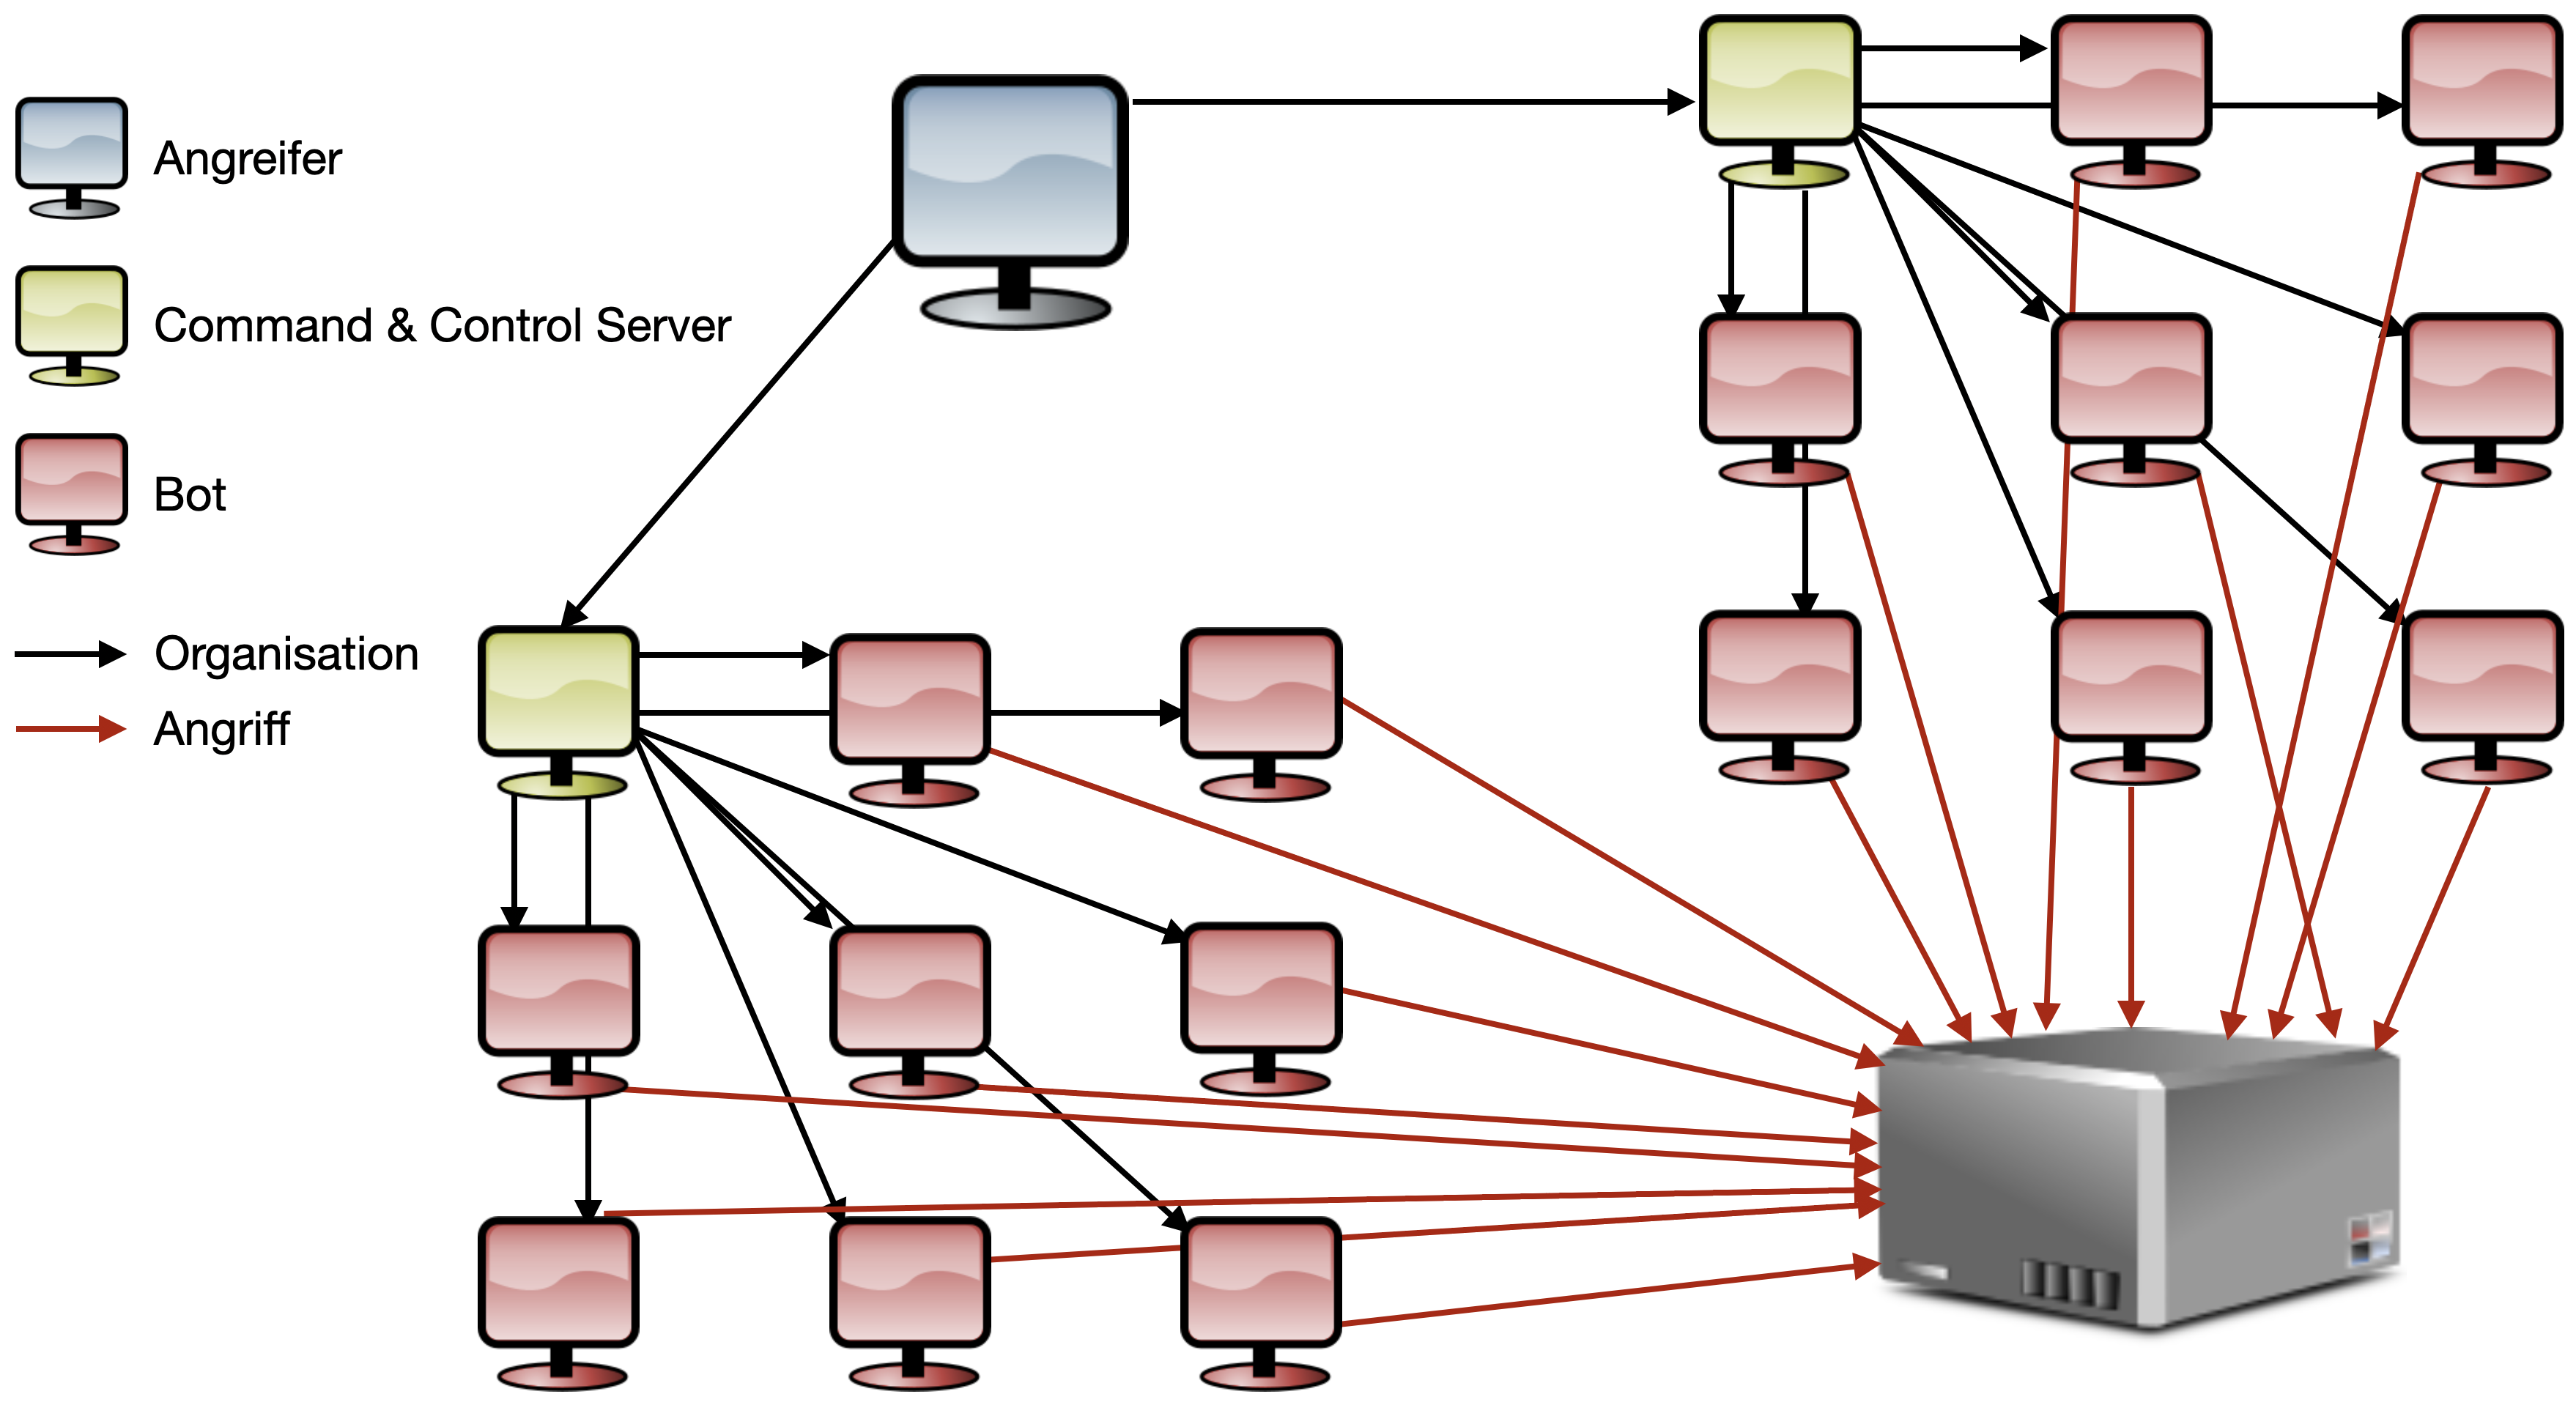
\includegraphics[width=\textwidth, center]{kapitel1/botnet}
		\caption[Schematischer Aufbau bei einem DDoS-Angriff mit einem Botnetz]{Schematischer Aufbau eines Botnetzes zur Durchführung eines DDoS-Angriffs}
		\label{img:botnet}
\end{figure}

Eine Analogie zu einem DDoS-Angriff aus dem realen Leben wäre die Benutzung von einem Bus. Spricht man sich hierbei ab, dass sehr viele Leute gleichzeitig versuchen in einen Bus einzusteigen, so bleibt kaum bis kein Platz mehr für die eigentlichen Fahrgäste. Das Ergebnis ist die Nichtverfügbarkeit eines Systems, in diesem Fall der Bus.
